\section{Langkah-Langkah Percobaan}
\subsection{Routing Statis IPv6}
\begin{enumerate}
      \item \textbf{Reset Router} \\
    Reset router ke kondisi awal dengan menghapus semua konfigurasi sebelumnya agar tidak terjadi konflik. Gunakan Winbox: masuk ke menu \texttt{System > Reset Configuration}, lalu centang \texttt{No Default Configuration}.

    \begin{figure}[H]
        \centering
        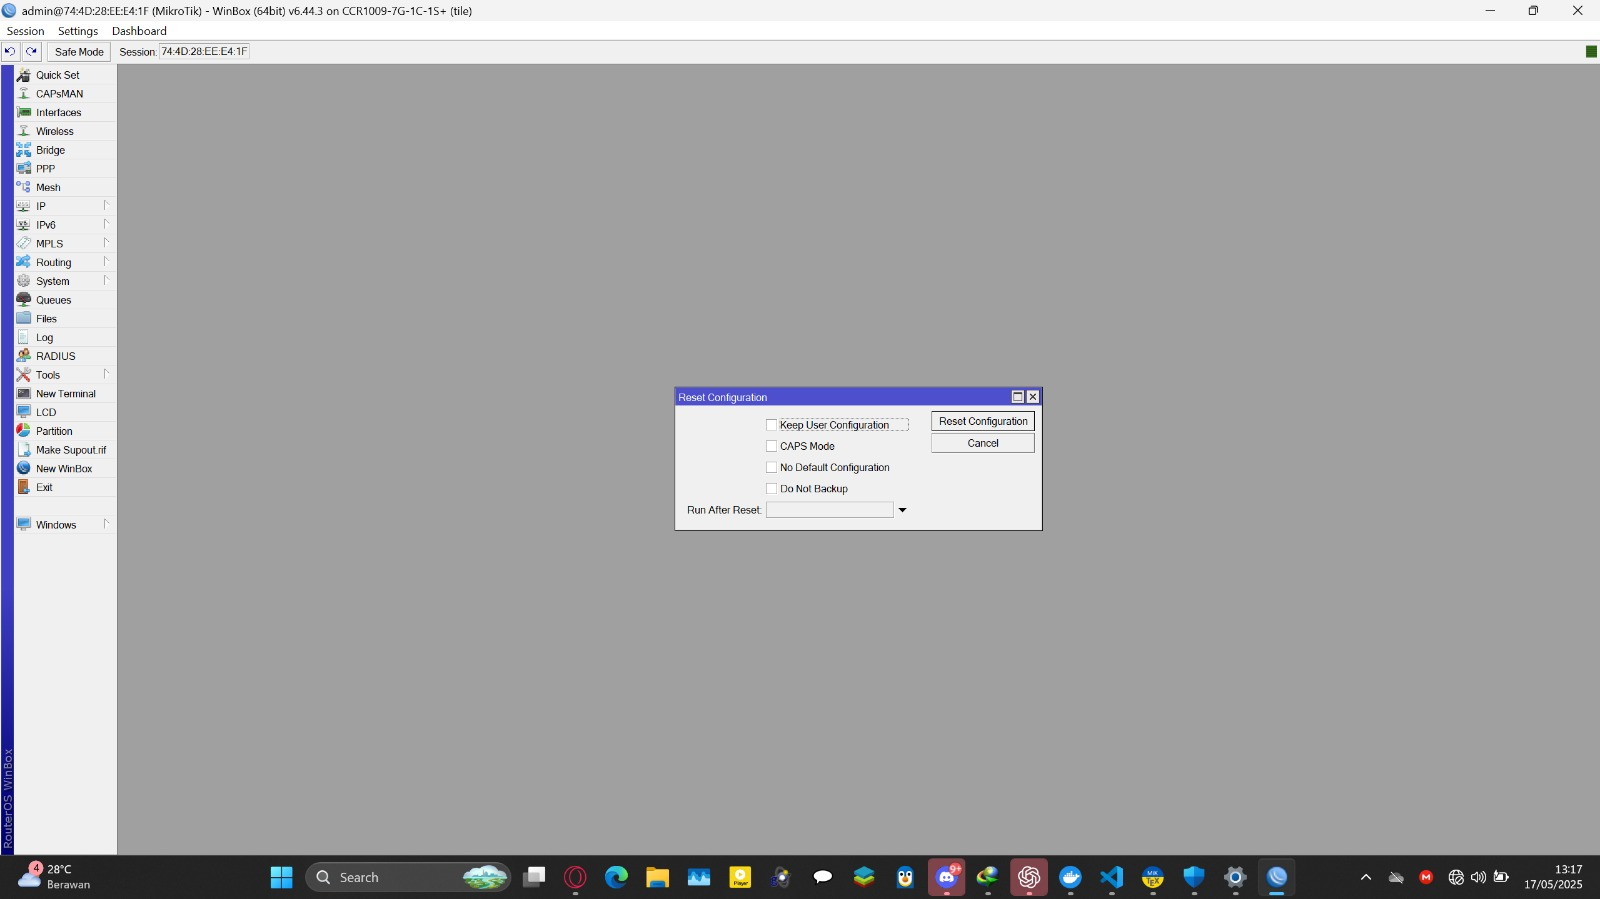
\includegraphics[width=0.5\linewidth]{P2/img/1 (4).jpg}
        \caption{Reset Router Menggunakan Winbox}
        \label{fig:gambar1}
    \end{figure}

    \item \textbf{Login ke Router} \\
    Login ke router menggunakan Winbox melalui MAC address atau IP default. Gunakan username \texttt{admin} tanpa password jika belum diatur.

    \begin{figure}[H]
        \centering
        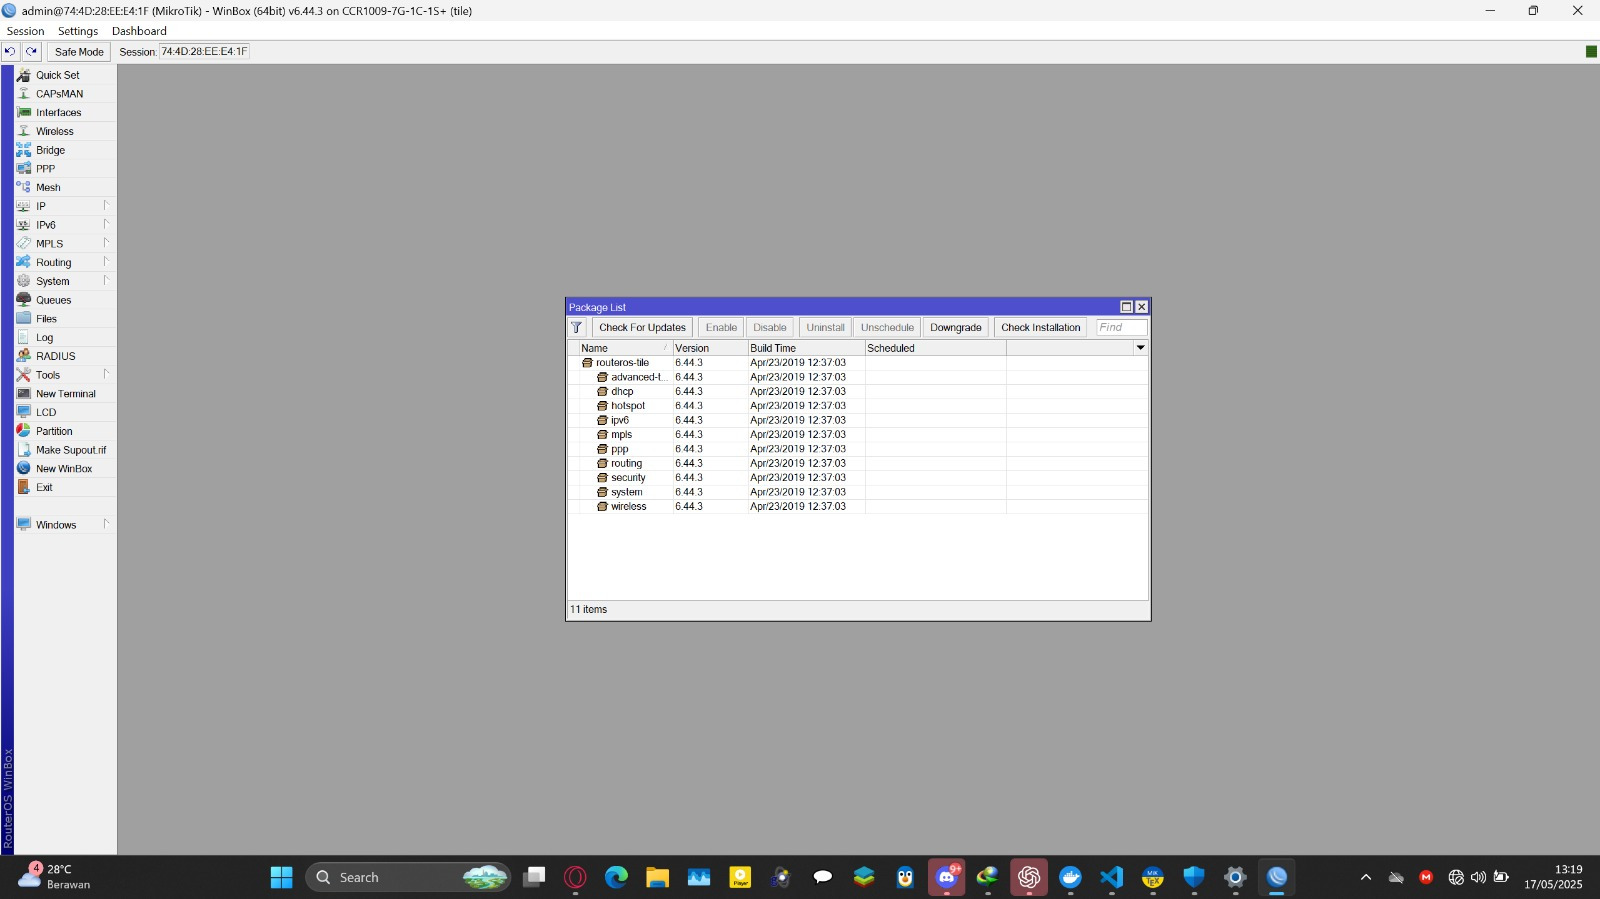
\includegraphics[width=0.5\linewidth]{P2/img/1 (6).jpg}
        \caption{Login ke Router dengan Winbox}
        \label{fig:gambar2}
    \end{figure}

    \item \textbf{Konfigurasi IP Address pada Ether1 (Router A dan B)} \\
    Tambahkan IP address pada \texttt{ether1} yang digunakan sebagai jalur antar-router:
    \begin{itemize}
        \item Router A: \texttt{ether1 = 2001:db8:1::1/64}
        \item Router B: \texttt{ether1 = 2001:db8:1::2/64}
    \end{itemize}

    \begin{figure}[H]
        \centering
        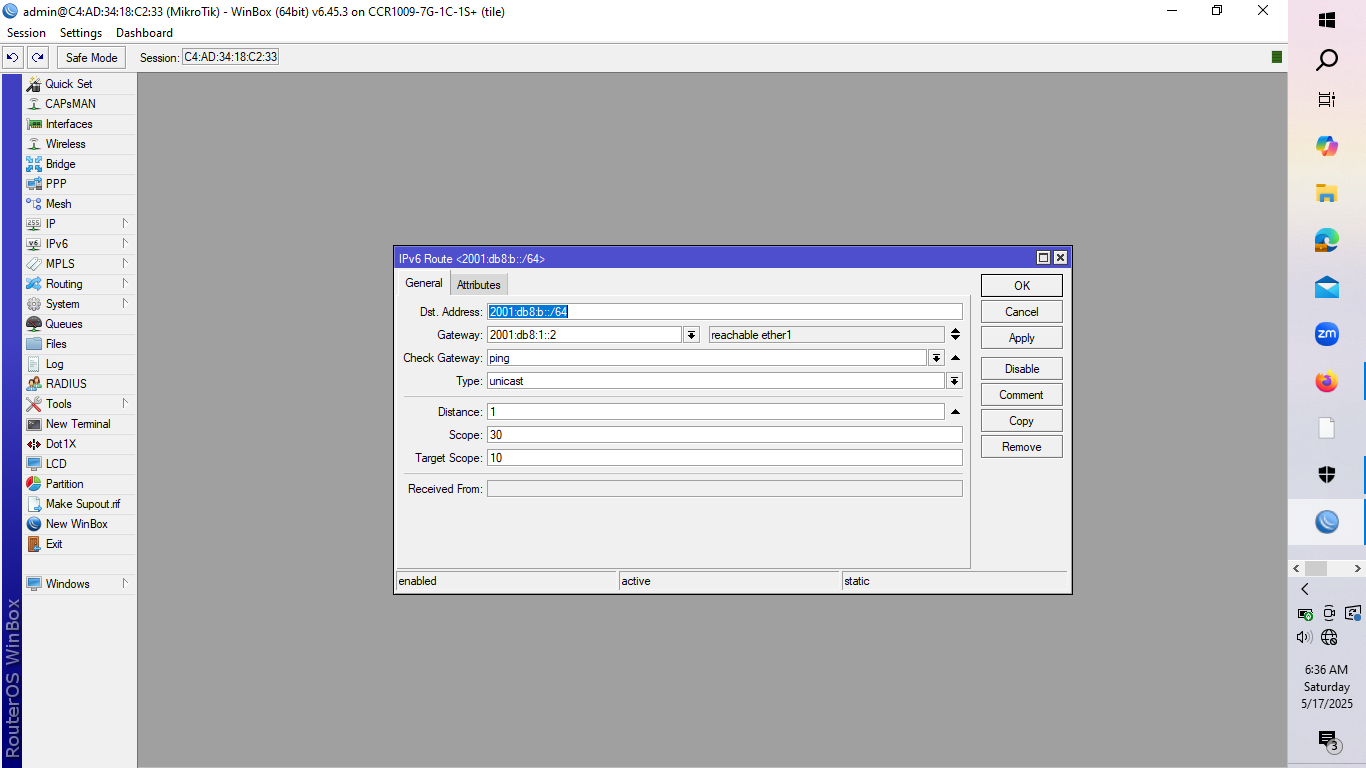
\includegraphics[width=0.5\linewidth]{P2/img/gambar3.png}
        \caption{Konfigurasi IP Ether1}
        \label{fig:gambar3}
    \end{figure}

    \item \textbf{Konfigurasi IP Address untuk Jaringan LAN (Router A dan B)} \\
    Tambahkan IP address pada \texttt{ether2} untuk koneksi ke laptop:
    \begin{itemize}
        \item Router A: \texttt{ether2 = 2001:db8:a::1/64}
        \item Router B: \texttt{ether2 = 2001:db8:b::1/64}
    \end{itemize}

    \begin{figure}[H]
        \centering
        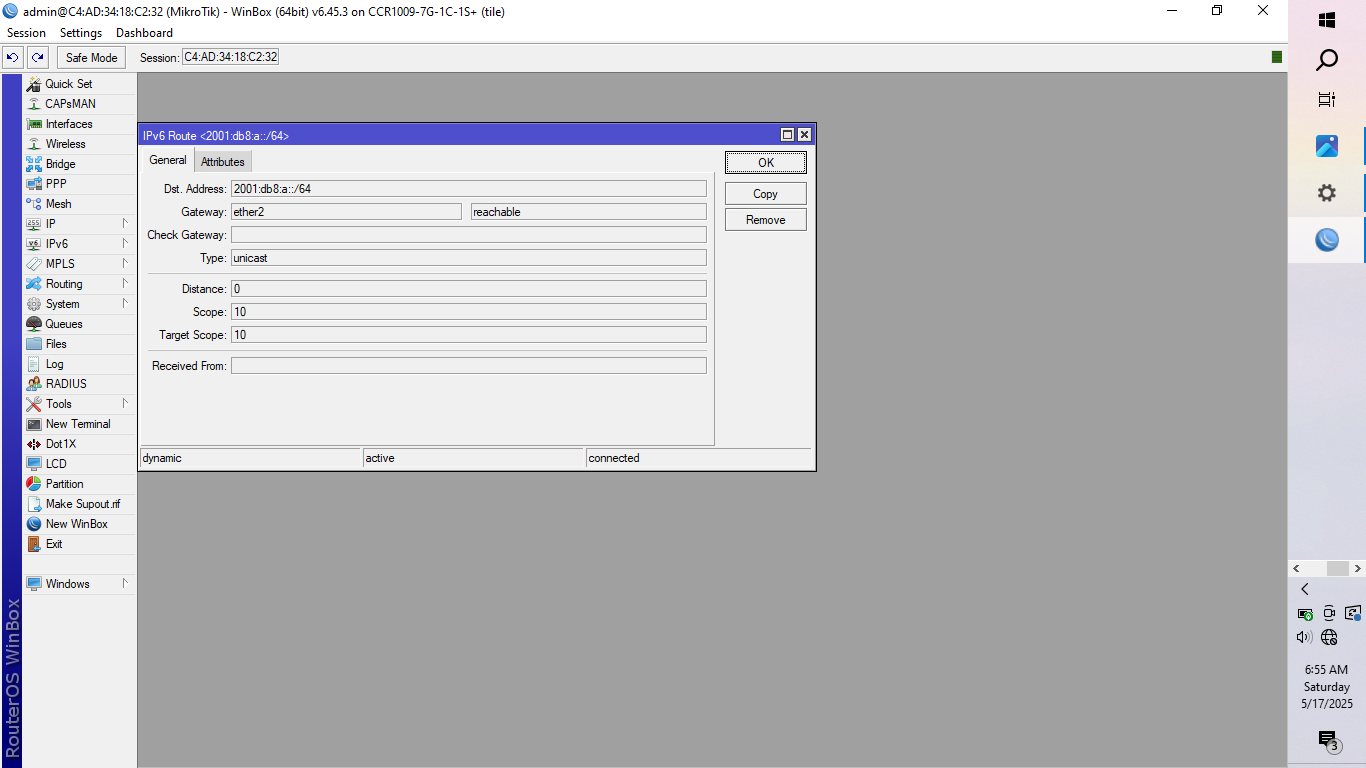
\includegraphics[width=0.5\linewidth]{P2/img/Screenshot (183).png}
        \caption{Konfigurasi IP Ether2}
        \label{fig:gambar4}
    \end{figure}

    \item \textbf{Konfigurasi Routing Statis (Router A dan B)} \\
    Tambahkan rute secara manual melalui \texttt{IPv6 > Routes}, lalu klik \texttt{"+"}:
    \begin{itemize}
        \item Router A:
        \begin{itemize}
            \item \texttt{Dst. Address: 2001:db8:b::/64}
            \item \texttt{Gateway: 2001:db8:1::2}
        \end{itemize}
        \item Router B:
        \begin{itemize}
            \item \texttt{Dst. Address: 2001:db8:a::/64}
            \item \texttt{Gateway: 2001:db8:1::1}
        \end{itemize}
    \end{itemize}

    \begin{figure}[H]
        \centering
        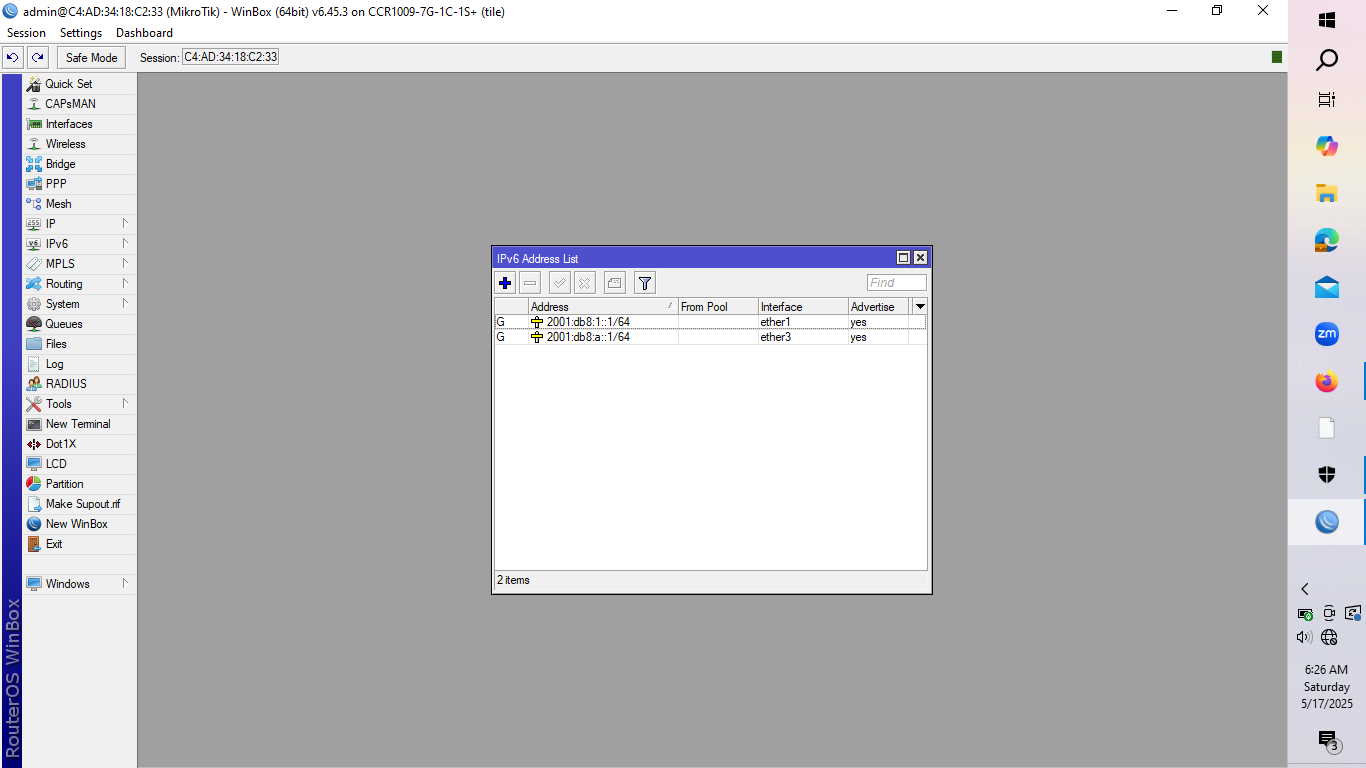
\includegraphics[width=0.5\linewidth]{P2/img/gambar2.png}
        \caption{Menambahkan Routing Statis}
        \label{fig:gambar5}
    \end{figure}

    \item \textbf{Test Koneksi Antar Router} \\
    Lakukan ping antar-router:
    \begin{itemize}
        \item Dari Router A: \texttt{ping 2001:db8:b::1}
        \item Dari Router B: \texttt{ping 2001:db8:a::1}
    \end{itemize}

    \begin{figure}[H]
        \centering
        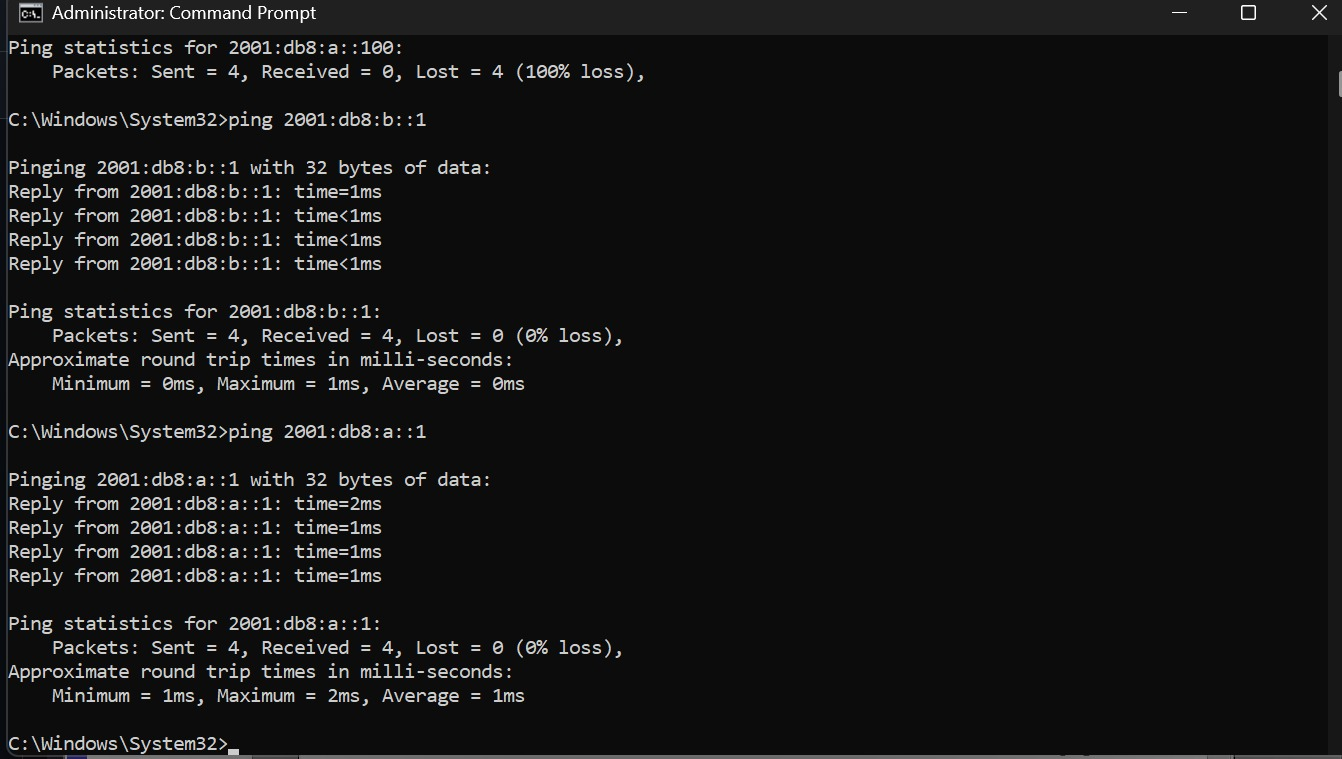
\includegraphics[width=0.5\linewidth]{P2/img/1 (11).jpg}
        \caption{Uji Ping Antar Router}
        \label{fig:gambar6}
    \end{figure}

    \item \textbf{Konfigurasi IP Address di Laptop} \\
    Tambahkan IP address secara manual di masing-masing laptop:
    \begin{itemize}
        \item Laptop terhubung ke Router A:
        \begin{itemize}
            \item IP: \texttt{2001:db8:a::100}
            \item Prefix: \texttt{/64}
            \item Gateway: \texttt{2001:db8:a::1}
            \item DNS: \texttt{2001:4860:4860::8888}
        \end{itemize}
        \item Laptop terhubung ke Router B:
        \begin{itemize}
            \item IP: \texttt{2001:db8:b::100}
            \item Prefix: \texttt{/64}
            \item Gateway: \texttt{2001:db8:b::1}
            \item DNS: \texttt{2001:4860:4860::8888}
        \end{itemize}
    \end{itemize}

    \begin{figure}[H]
        \centering
        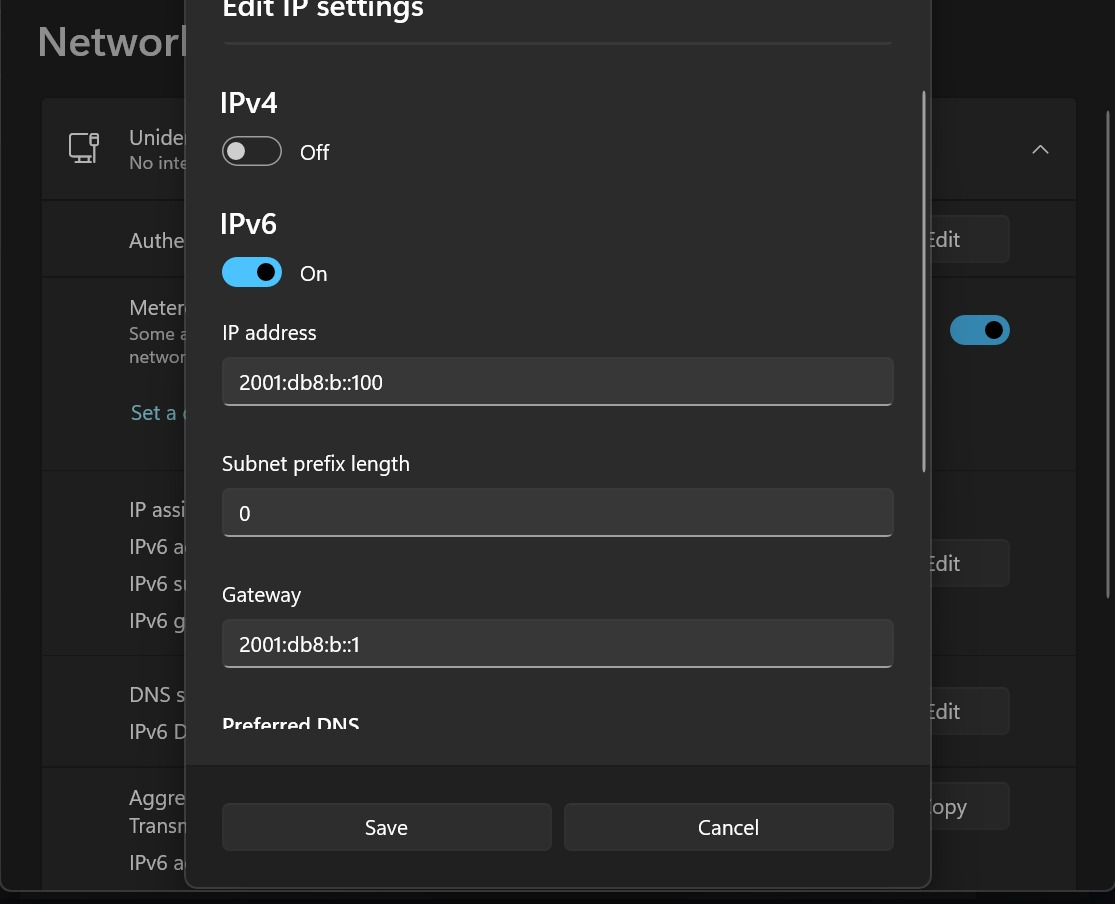
\includegraphics[width=0.5\linewidth]{P2/img/1 (9).jpg}
        \caption{Konfigurasi IP di Laptop}
        \label{fig:gambar7}
    \end{figure}

    \item \textbf{Uji Koneksi Antar Laptop} \\
    Lakukan ping dari Laptop 1 ke Laptop 2:
    \begin{itemize}
        \item \texttt{ping 2001:db8:b::100}
    \end{itemize}
    Jika berhasil, routing sudah berjalan dengan baik.

    \begin{figure}[H]
        \centering
        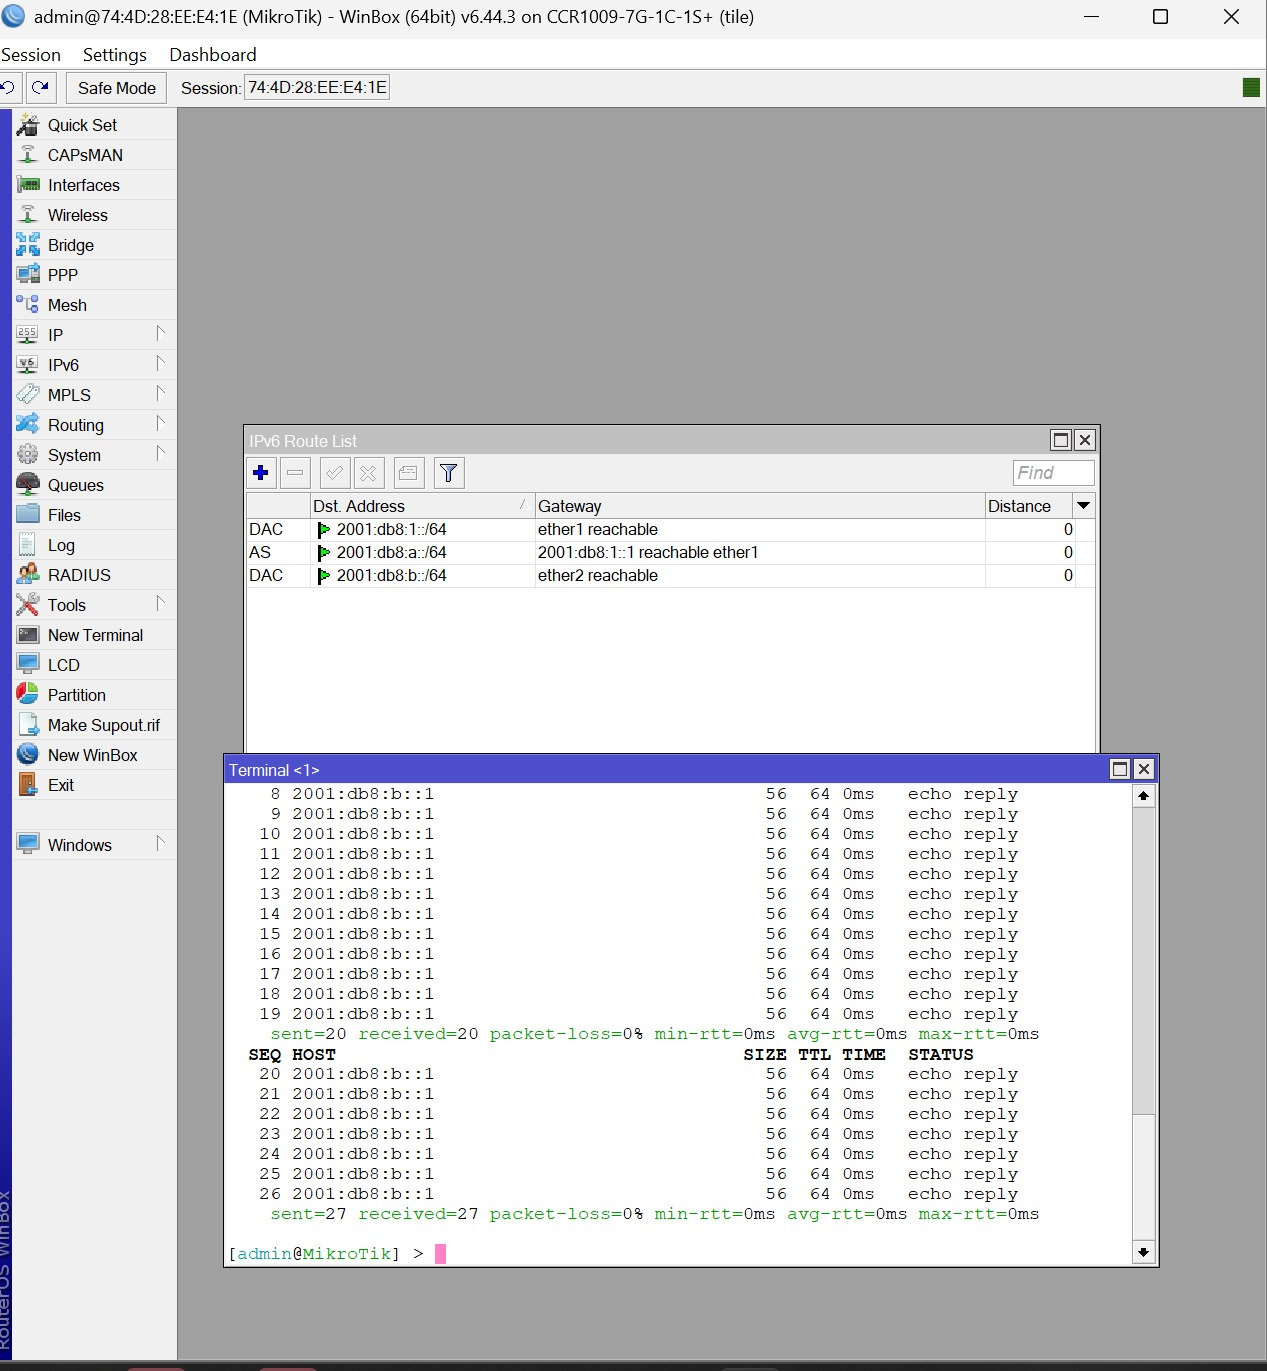
\includegraphics[width=0.5\linewidth]{P2/img/1 (13).jpg}
        \caption{Ping Antar Laptop}
        \label{fig:gambar8}
    \end{figure}
\end{enumerate}

\subsection{Routing Dinamis IPv6}
\begin{enumerate}
    \item \textbf{Reset Router:} Kembalikan router ke kondisi awal tanpa konfigurasi.
    \begin{figure}[H]
        \centering
        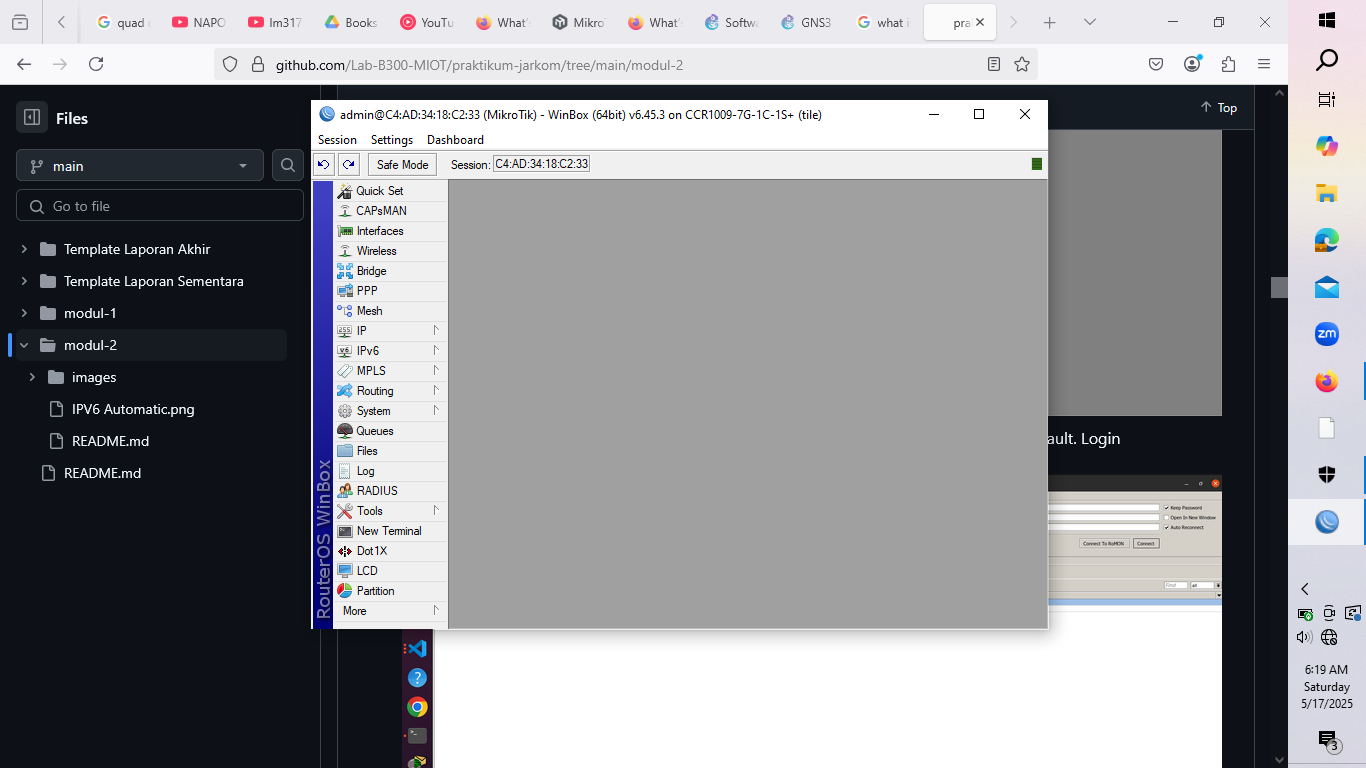
\includegraphics[width=0.5\linewidth]{P2/img/gambar1.png}
        \caption{Reset Router}
        \label{fig:gambar1}
    \end{figure}

    \item \textbf{Login Router:} Akses router via Winbox sebagai admin.
    \begin{figure}[H]
        \centering
        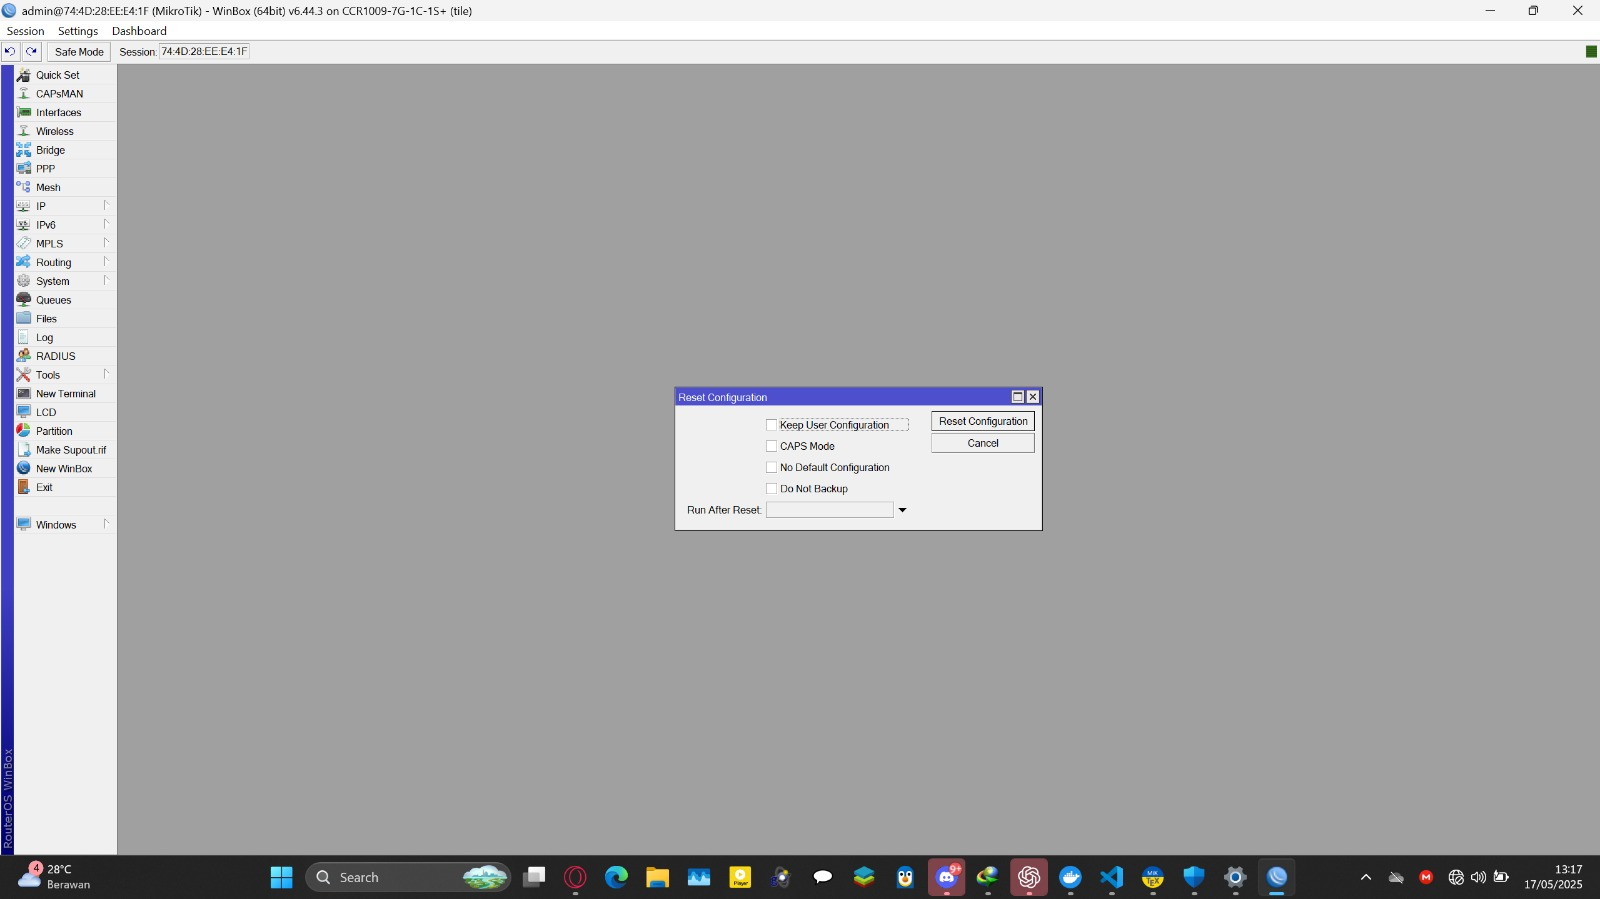
\includegraphics[width=0.5\linewidth]{P2/img/1 (4).jpg}
        \caption{Login ke Router}
        \label{fig:gambar2}
    \end{figure}

    \item \textbf{Atur Alamat IP:} Tambahkan alamat IPv6 pada antarmuka antar-router dan LAN.
    \begin{figure}[H]
        \centering
        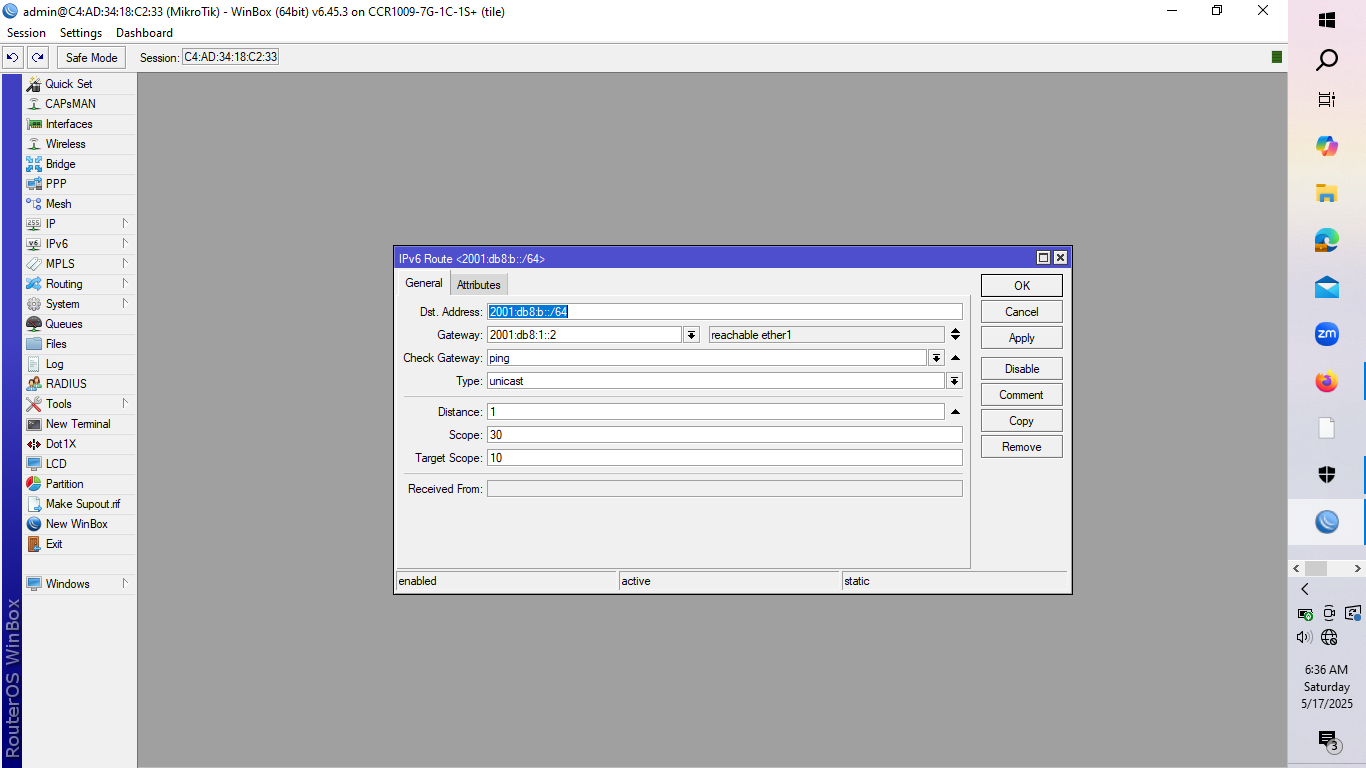
\includegraphics[width=0.5\linewidth]{P2/img/gambar3.png}
        \caption{Konfigurasi IP pada Antarmuka}
        \label{fig:gambar3}
    \end{figure}

    \item \textbf{Aktifkan OSPFv3:}
    \begin{itemize}
        \item Buat \textit{instance} OSPF dengan ID unik.
        \item Tambahkan \textit{area} backbone (ID: 0.0.0.0).
        \item Masukkan antarmuka (ether1 dan ether2) ke area tersebut.
    \end{itemize}
    \begin{figure}[H]
        \centering
        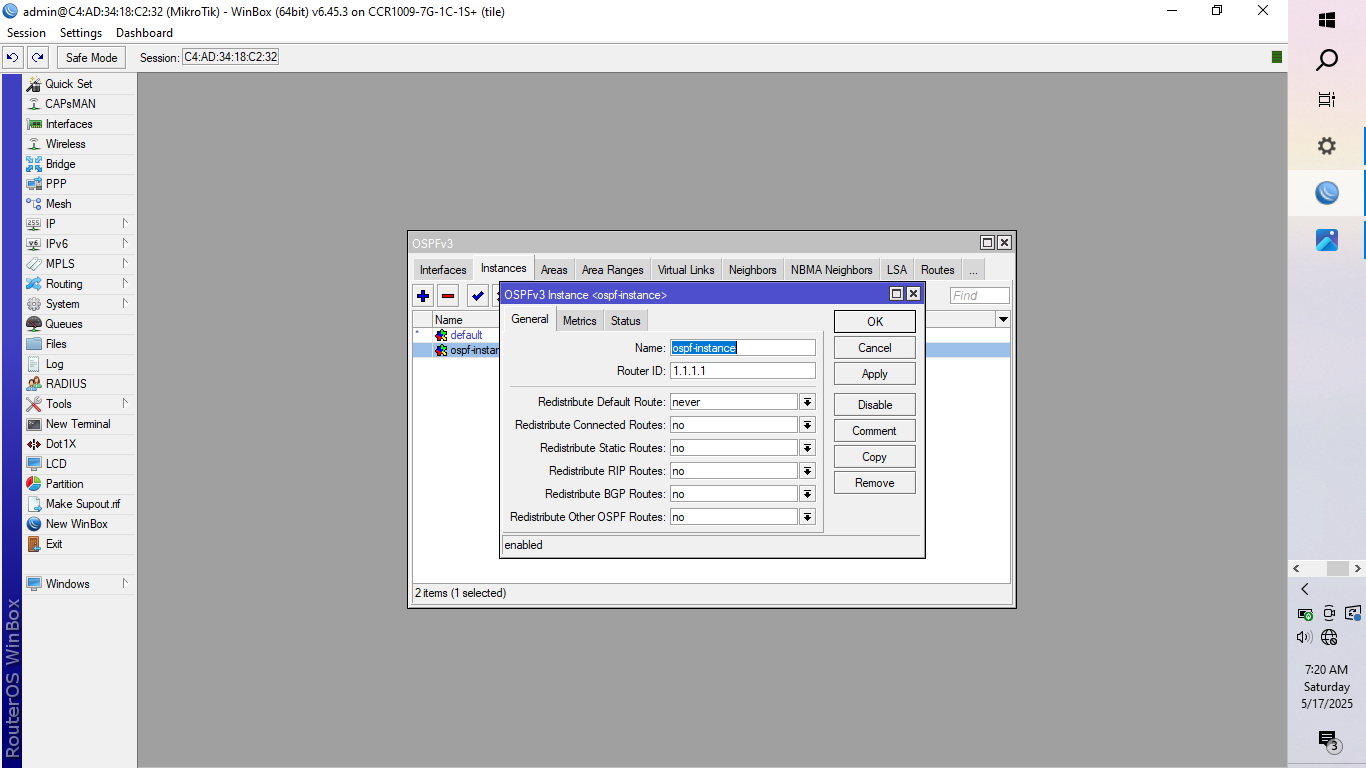
\includegraphics[width=0.5\linewidth]{P2/img/gambar5.png}
        \caption{Pengaturan OSPFv3}
        \label{fig:gambar4}
    \end{figure}

    \item \textbf{Cek Neighbor dan Rute:} Pastikan tetangga OSPF muncul dan rute dinamis terbentuk.
    \begin{figure}[H]
        \centering
        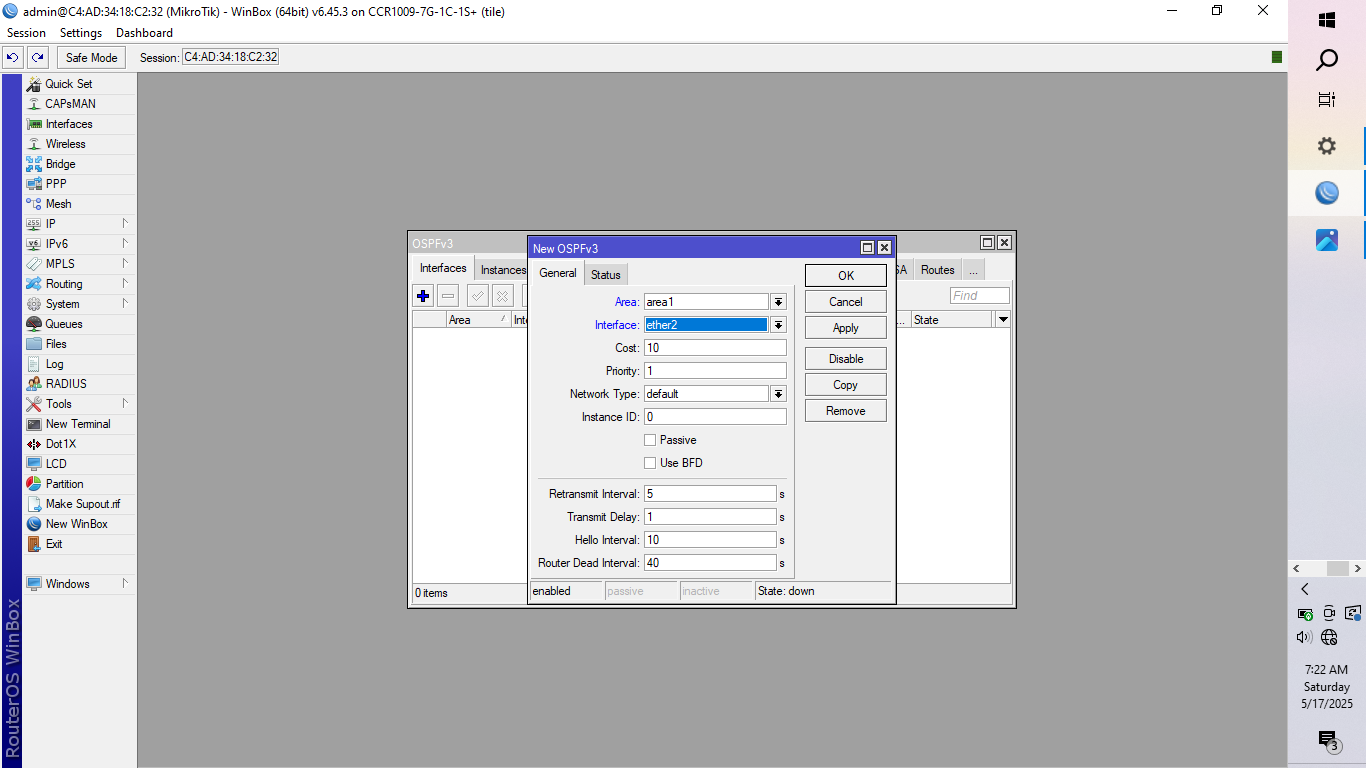
\includegraphics[width=0.5\linewidth]{P2/img/gambar6.png}
        \caption{Cek Neighbor dan Routing}
        \label{fig:gambar5}
    \end{figure}

    \item \textbf{Konfigurasi Laptop:} Atur alamat IPv6, prefix, gateway, dan DNS secara manual.
    \begin{figure}[H]
        \centering
        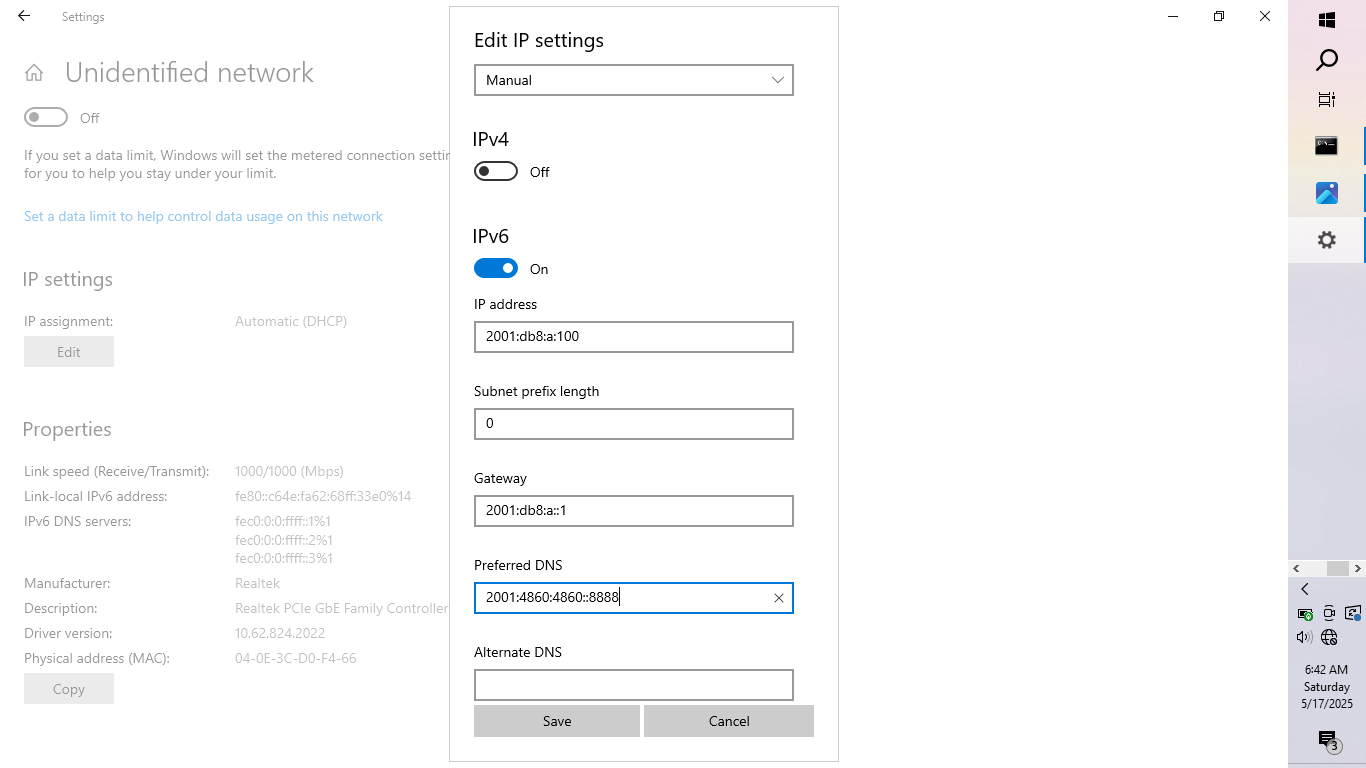
\includegraphics[width=0.5\linewidth]{P2/img/gambar4.png}
        \caption{Konfigurasi IP di Laptop}
        \label{fig:gambar6}
    \end{figure}

    \item \textbf{Uji Koneksi:} Lakukan ping antar perangkat untuk memastikan konektivitas.
    \begin{figure}[H]
        \centering
        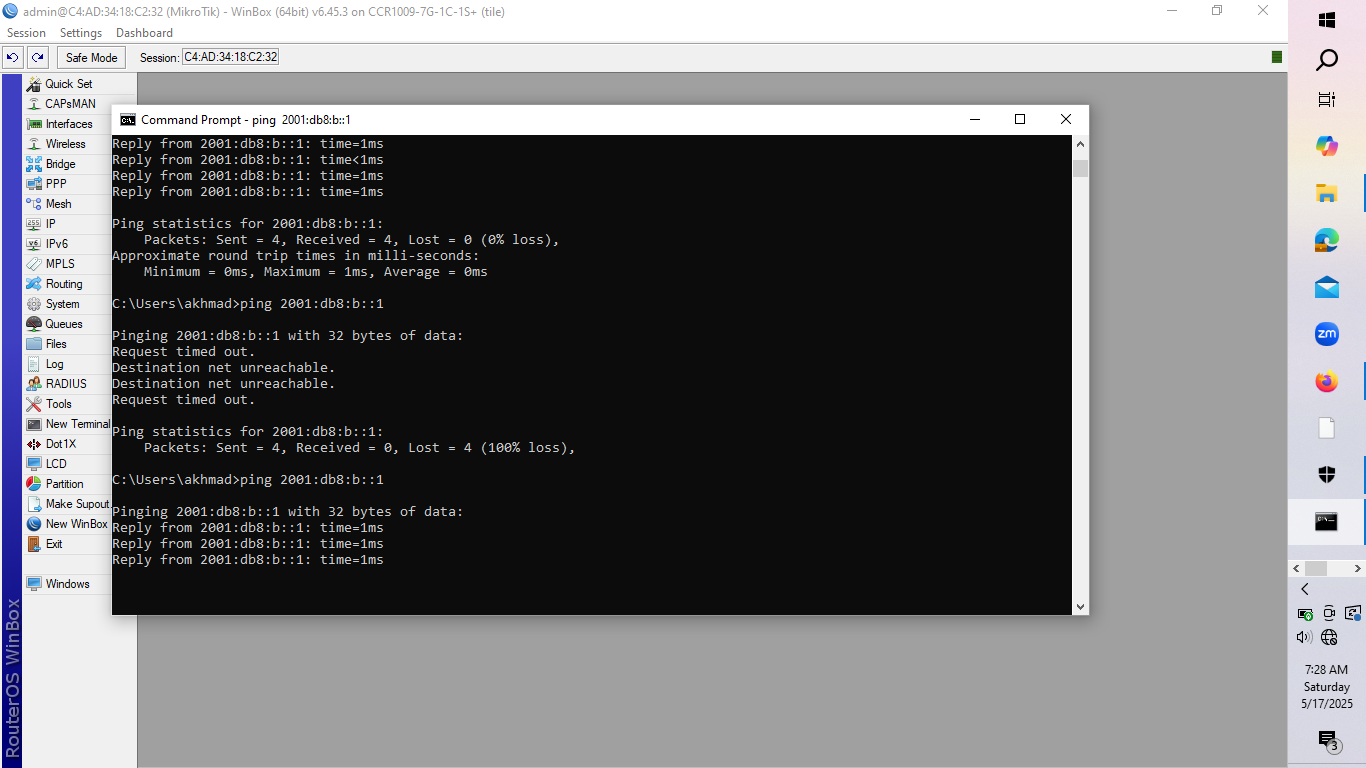
\includegraphics[width=0.5\linewidth]{P2/img/ping1.png}
        \caption{Uji Koneksi Antar Laptop}
        \label{fig:gambar7}
    \end{figure}
\end{enumerate}

\section{Analisis Hasil Percobaan}
Berdasarkan pengujian terhadap routing statis IPv6, terlihat bahwa seluruh laptop dapat saling terhubung dan berhasil melakukan ping ke router. Hal ini membuktikan bahwa konfigurasi routing statis IPv6 telah dilakukan dengan benar. Sementara itu, pada uji coba routing dinamis IPv6, semua perangkat juga menunjukkan konektivitas yang baik satu sama lain serta ke router, menandakan bahwa penerapan routing dinamis IPv6 berjalan dengan lancar.

\section{Hasil Tugas Modul}
\subsection{Simulasikan Konfigurasi Praktikum P2 di atas mengenai Routing Dinamis dan Statis IPV6 menggunakan GNS3.}

\subsection{Topologi Jaringan}
Topologi yang digunakan terdiri dari dua buah PC dan dua buah router yang saling terhubung secara point-to-point:

\begin{center}
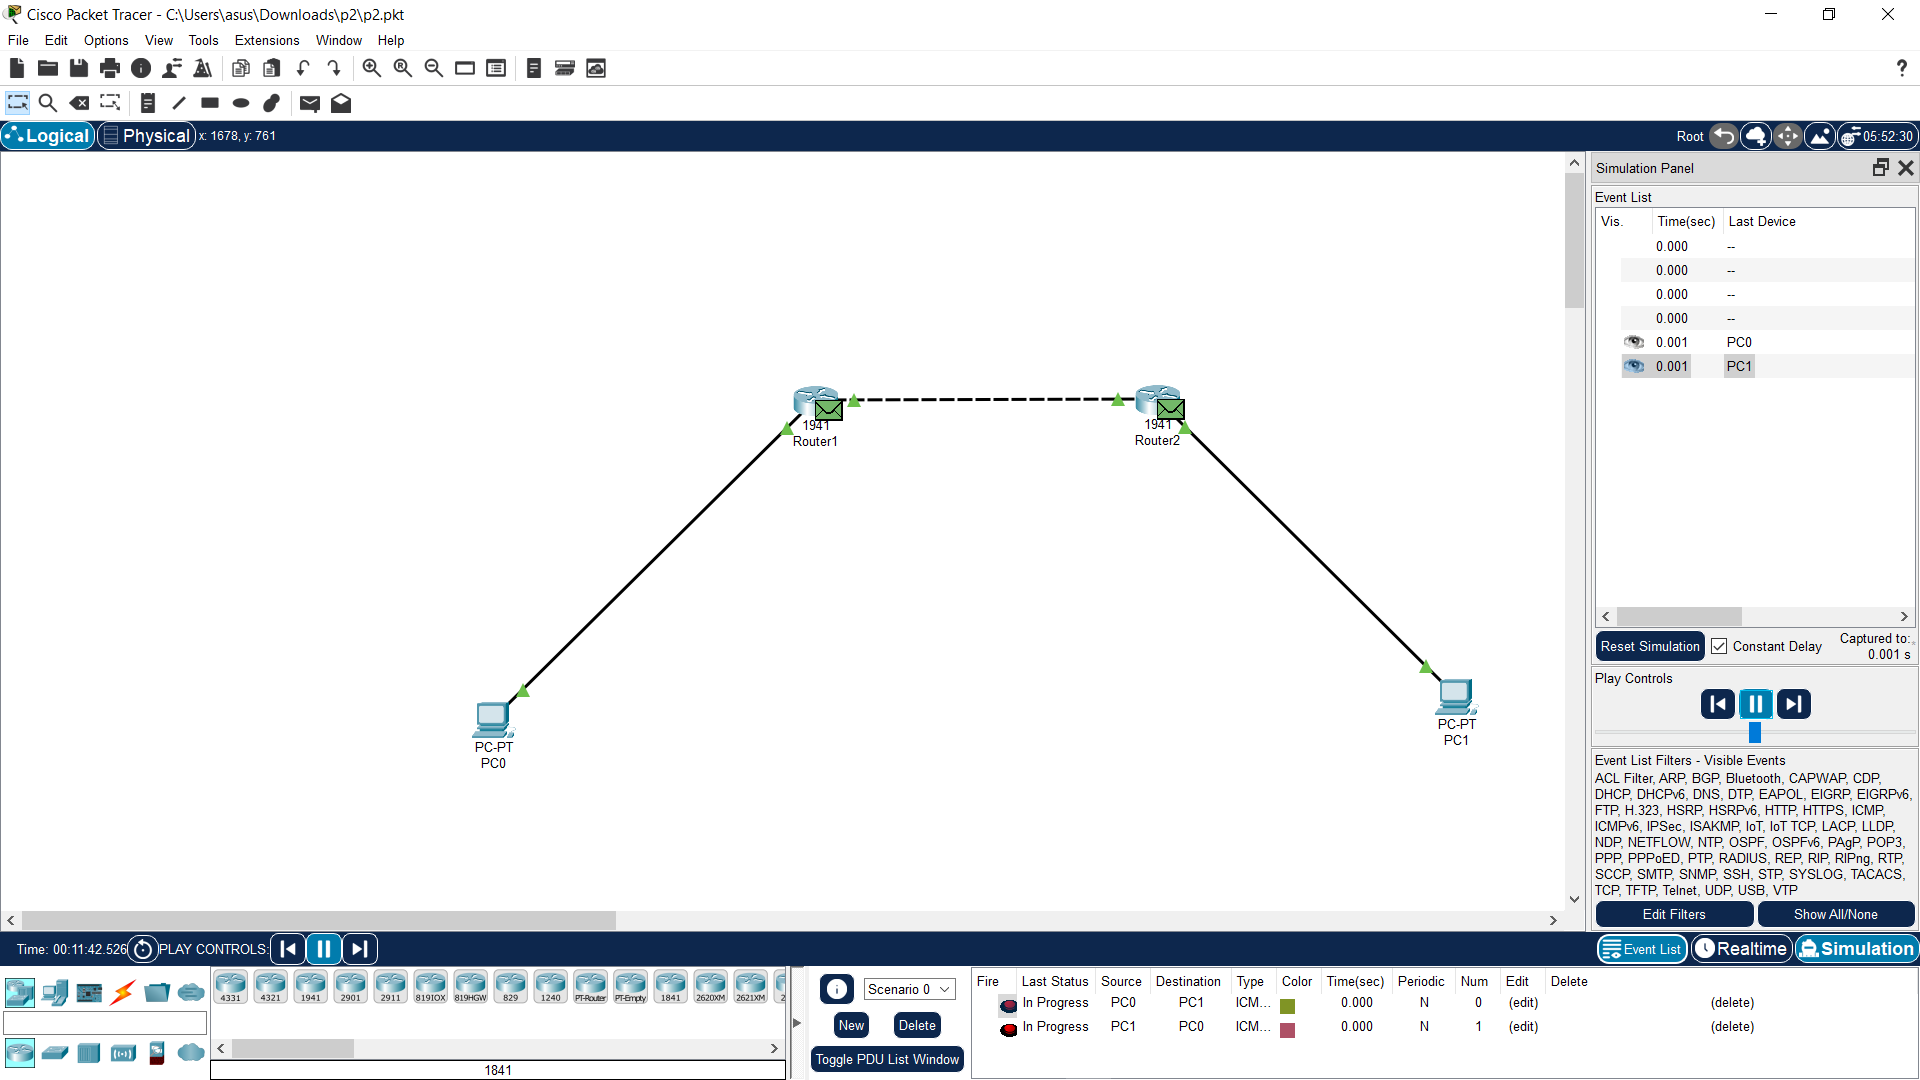
\includegraphics[width=0.8\textwidth]{P2/img/paket.png}
\end{center}

\begin{itemize}
    \item PC0 --- Router1 --- Router2 --- PC1
    \item Koneksi antar perangkat menggunakan alamat IPv6
\end{itemize}

\subsection{Routing Statis IPv6}
Pada metode routing statis, setiap router dikonfigurasi secara manual agar dapat saling mengetahui jaringan yang tidak langsung terhubung.

\begin{itemize}
    \item \textbf{Router1}
    \begin{itemize}
        \item ether1: \texttt{2001:db8:1::1/64} (ke Router2)
        \item ether2: \texttt{2001:db8:a::1/64} (ke PC0)
    \end{itemize}
    \item \textbf{Router2}
    \begin{itemize}
        \item ether1: \texttt{2001:db8:1::2/64} (ke Router1)
        \item ether2: \texttt{2001:db8:b::1/64} (ke PC1)
    \end{itemize}
    \item \textbf{Routing Table Manual}
    \begin{itemize}
        \item Di Router1:
        \begin{quote}
            Dst Address: \texttt{2001:db8:b::/64} \\
            Gateway: \texttt{2001:db8:1::2}
        \end{quote}
        \item Di Router2:
        \begin{quote}
            Dst Address: \texttt{2001:db8:a::/64} \\
            Gateway: \texttt{2001:db8:1::1}
        \end{quote}
    \end{itemize}
\end{itemize}

\subsection{Routing Dinamis IPv6 (OSPFv3)}
Pada metode ini, digunakan protokol OSPFv3 yang memungkinkan router saling bertukar informasi routing secara otomatis.

\begin{enumerate}
    \item Buat \textbf{Instance OSPFv3}
    \item Tambahkan \textbf{Area Backbone (0.0.0.0)}
    \item Tambahkan interface ether1 dan ether2 ke dalam area OSPF
    \item Cek tetangga (\textit{neighbors}) OSPF dan tabel routing
\end{enumerate}

\subsection{Konfigurasi PC}
Masing-masing PC diberi alamat IPv6 secara statik:

\begin{itemize}
    \item \textbf{PC0}
    \begin{itemize}
        \item IP: \texttt{2001:db8:a::100/64}
        \item Gateway: \texttt{2001:db8:a::1}
    \end{itemize}
    \item \textbf{PC1}
    \begin{itemize}
        \item IP: \texttt{2001:db8:b::100/64}
        \item Gateway: \texttt{2001:db8:b::1}
    \end{itemize}
\end{itemize}

\subsection{Pengujian}
Dilakukan uji konektivitas menggunakan \texttt{ping} dari PC0 ke PC1 dan sebaliknya. Jika koneksi berhasil, maka konfigurasi routing IPv6 baik statis maupun dinamis dinyatakan berhasil.

\subsection{Analisis}
\begin{itemize}
    \item Routing statis IPv6 cocok digunakan untuk jaringan kecil yang topologinya tidak sering berubah.
    \item Routing dinamis IPv6 seperti OSPFv3 lebih efisien untuk jaringan besar karena mampu menyesuaikan perubahan topologi secara otomatis.
    \item Simulasi ini membuktikan bahwa kedua metode routing dapat diterapkan secara efektif pada jaringan IPv6.
\end{itemize}

\section{Kesimpulan}
Berdasarkan hasil percobaan yang telah dilakukan, dapat disimpulkan bahwa baik routing statis maupun routing dinamis IPv6 dapat berjalan dengan baik dalam jaringan komputer. Routing statis IPv6 lebih cocok diterapkan pada jaringan berskala kecil yang jarang mengalami perubahan topologi. Sementara itu, routing dinamis IPv6 lebih sesuai untuk jaringan yang luas dan sering mengalami perubahan topologi. Dibandingkan dengan routing statis, routing dinamis IPv6 lebih efisien dan lebih mudah dalam pengelolaannya karena mampu menyesuaikan secara otomatis terhadap perubahan topologi jaringan. Dalam penerapan routing dinamis IPv6, digunakan protokol OSPF yang mampu menyesuaikan diri secara otomatis terhadap perubahan struktur jaringan.

\section{Lampiran}
\subsection{Dokumentasi Saat Praktikum}
\begin{figure}[H]
    \centering
    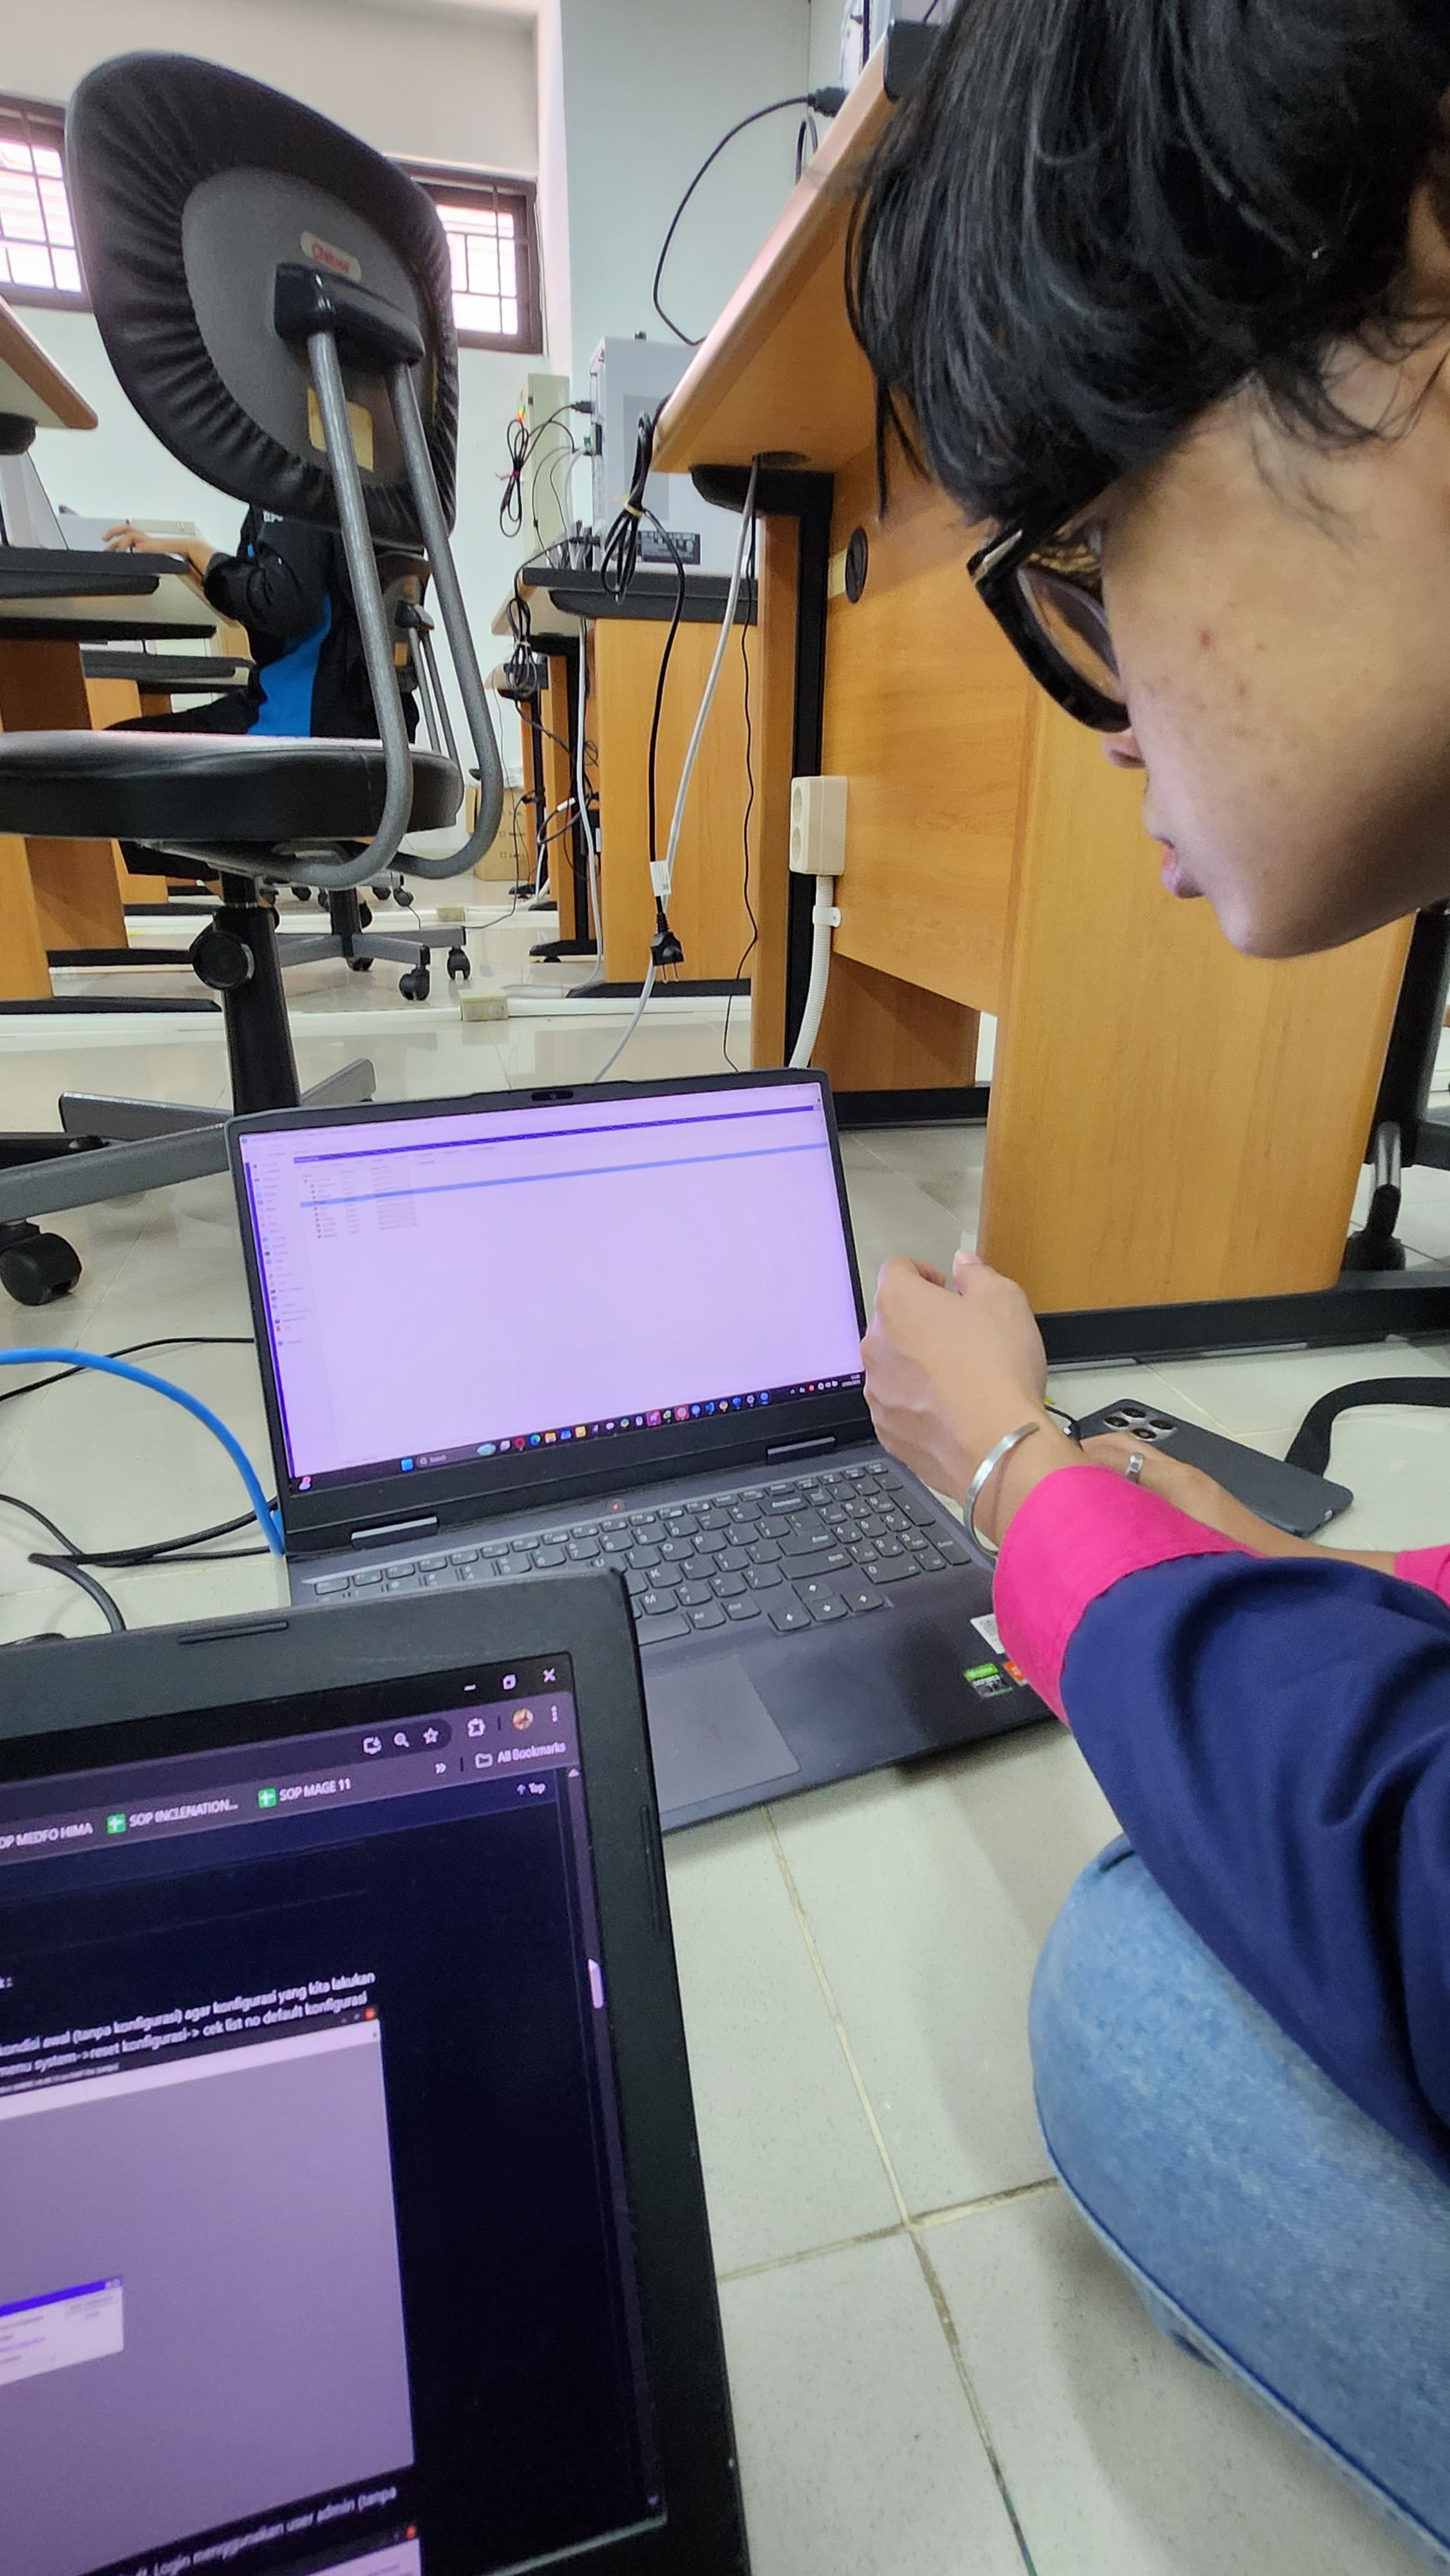
\includegraphics[width=0.3\textwidth]{P2/img/dokum1.jpg}
    \caption{Dokumentasi saat merouting IPv6 di Laptop}
    \label{fig:labelgambar}
\end{figure}
\begin{figure}[H]
    \centering
    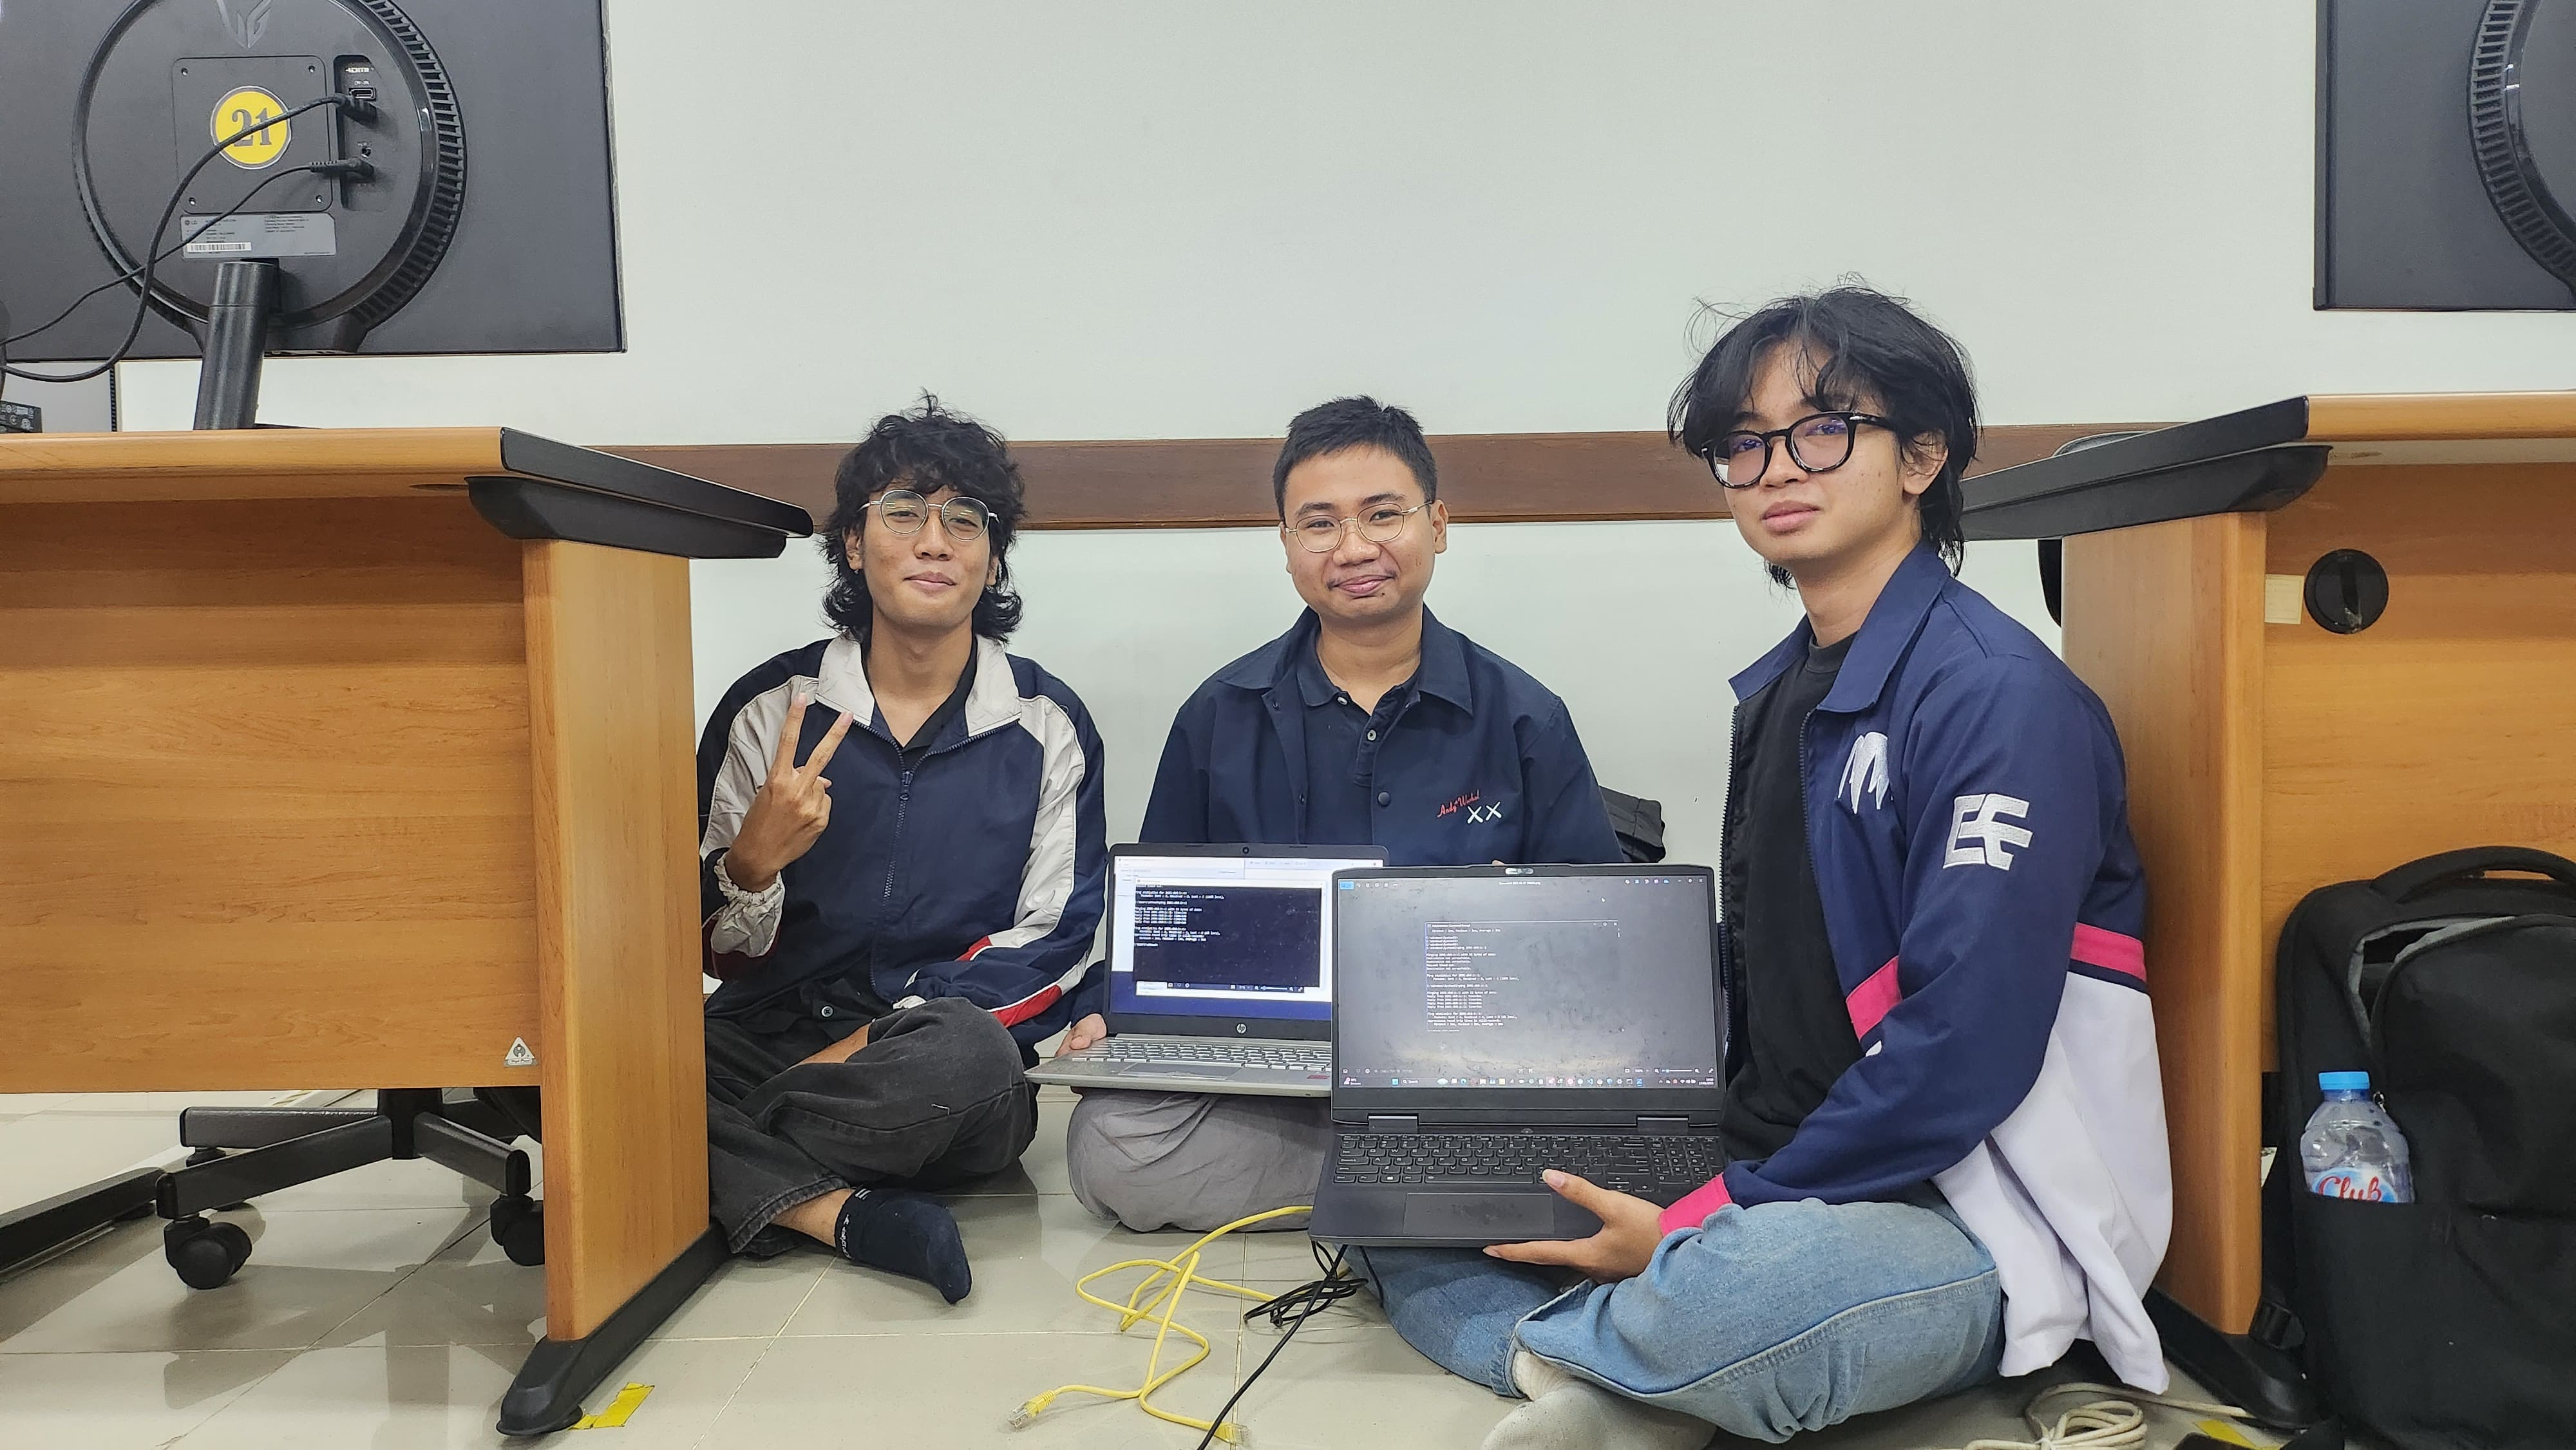
\includegraphics[width=0.5\textwidth]{P2/img/dokum2.jpg}
    \caption{Dokumentasi setelah berhasil routing IPv6}
    \label{fig:labelgambar}
\end{figure}